\documentclass[12pt, letterpaper]{article}


\usepackage[utf8]{inputenc}
\usepackage[T1]{fontenc}
\usepackage{geometry}
\usepackage{graphicx}
\usepackage{float}
\usepackage{booktabs}
\usepackage{array}
\usepackage{hyperref}
\usepackage{xcolor}
\usepackage{tikz}
\usepackage{enumitem}
\usepackage{amsmath}
\usepackage{amssymb}
\usepackage{listings}

\usetikzlibrary{arrows.meta, positioning, shapes.geometric}

\geometry{
	left=2.5cm,
	right=2.5cm,
	top=2.5cm,
	bottom=2.5cm
}

\hypersetup{
	colorlinks=true,
	linkcolor=black,
	urlcolor=blue,
	citecolor=black
}

\lstset{
	basicstyle=\ttfamily\small,
	breaklines=true,
	frame=single,
	backgroundcolor=\color{gray!5},
	columns=fullflexible
}

\title{
	\textbf{LeerIA: Plataforma Inteligente para el Estudio Asistido por Documentos}\\
	\large Proyecto Final --- Introducción a la Inteligencia Artificial 2026-1
}

\author{
	Simón Sloan García Villa\\
	Universidad EAFIT
}

\date{2026-1}

\begin{document}
	
	\maketitle
	
	\begin{abstract}
		LeerIA es una plataforma web basada en inteligencia artificial que permite convertir documentos académicos en una experiencia interactiva de estudio. El sistema permite subir archivos, procesarlos, extraer fragmentos relevantes, responder preguntas mediante un asistente conversacional y generar materiales de apoyo como resúmenes, quizzes, flashcards y guiones de video. La solución integra procesamiento de lenguaje natural, recuperación de información, embeddings semánticos y modelos generativos de lenguaje dentro de una arquitectura web compuesta por un frontend en React, un backend en FastAPI y persistencia en Supabase. El objetivo principal es ayudar a estudiantes a estudiar documentos extensos de manera más eficiente, personalizada y contextual.
	\end{abstract}
	\newpage
	\tableofcontents
	\newpage
	

	\section{Planteamiento del Problema}

	
	En contextos universitarios, los estudiantes suelen enfrentarse a grandes volúmenes de información en forma de PDFs, apuntes, presentaciones, lecturas y documentos técnicos. El proceso tradicional de estudio exige leer, subrayar, resumir, crear preguntas, identificar conceptos clave y preparar repasos de forma manual. Esta tarea puede ser lenta, repetitiva y poco personalizada.
	
	Además, muchos estudiantes no solo necesitan leer el material, sino también interactuar con él: hacer preguntas, pedir explicaciones, generar ejercicios, construir flashcards y comprobar su comprensión antes de exámenes o sustentaciones. Sin embargo, las herramientas tradicionales de lectura de documentos no suelen ofrecer una experiencia integrada que combine carga de archivos, conversación contextual y generación automática de material de estudio.
	
	El problema abordado por este proyecto es:
	
	\begin{quote}
		\textit{¿Cómo diseñar una plataforma inteligente que permita a un estudiante cargar documentos académicos, conversar con ellos y generar materiales de estudio personalizados usando técnicas de inteligencia artificial?}
	\end{quote}
	
	LeerIA surge como una solución a este problema. La aplicación permite al usuario organizar documentos por materias, crear conversaciones asociadas a cada materia, hacer preguntas sobre el contenido y generar materiales de estudio basados en los documentos procesados.
	
	La motivación principal es mejorar la eficiencia del aprendizaje, reducir la carga manual de preparación académica y ofrecer una interfaz funcional que integre procesamiento documental, recuperación semántica y generación de lenguaje natural.
	

	\section{Objetivo General}

	
	Desarrollar una plataforma web inteligente llamada \textbf{LeerIA} que permita a los estudiantes cargar documentos académicos, procesarlos mediante técnicas de procesamiento de lenguaje natural y utilizar modelos generativos para responder preguntas y crear materiales de estudio como resúmenes, quizzes, flashcards y guiones de video.
	

	\section{Metodología}

	
	La metodología del proyecto se basó en el desarrollo incremental de una aplicación web con componentes de inteligencia artificial. El proceso general se dividió en las siguientes fases:
	
	\begin{enumerate}
		\item \textbf{Definición del problema}: identificación de la necesidad de estudiar documentos académicos de forma más interactiva.
		\item \textbf{Diseño de arquitectura}: separación entre frontend, backend, base de datos, almacenamiento y servicios de IA.
		\item \textbf{Carga y gestión documental}: implementación de subida de archivos y organización por materias.
		\item \textbf{Procesamiento de documentos}: extracción de texto, división en fragmentos y almacenamiento estructurado.
		\item \textbf{Recuperación de información}: búsqueda de fragmentos relevantes según la pregunta o el tipo de material a generar.
		\item \textbf{Generación con modelo de lenguaje}: uso de un modelo generativo para responder preguntas o crear materiales de estudio.
		\item \textbf{Diseño de interfaz}: creación de una interfaz web funcional con panel de materias, conversaciones, documentos y herramientas de estudio.
		\item \textbf{Pruebas funcionales}: validación manual del flujo completo desde carga de documento hasta generación de respuestas y materiales.
	\end{enumerate}
	
	\subsection{Diagrama de Flujo del Proceso}
	
	\begin{figure}[H]
		\centering
		\resizebox{0.95\textwidth}{!}{
			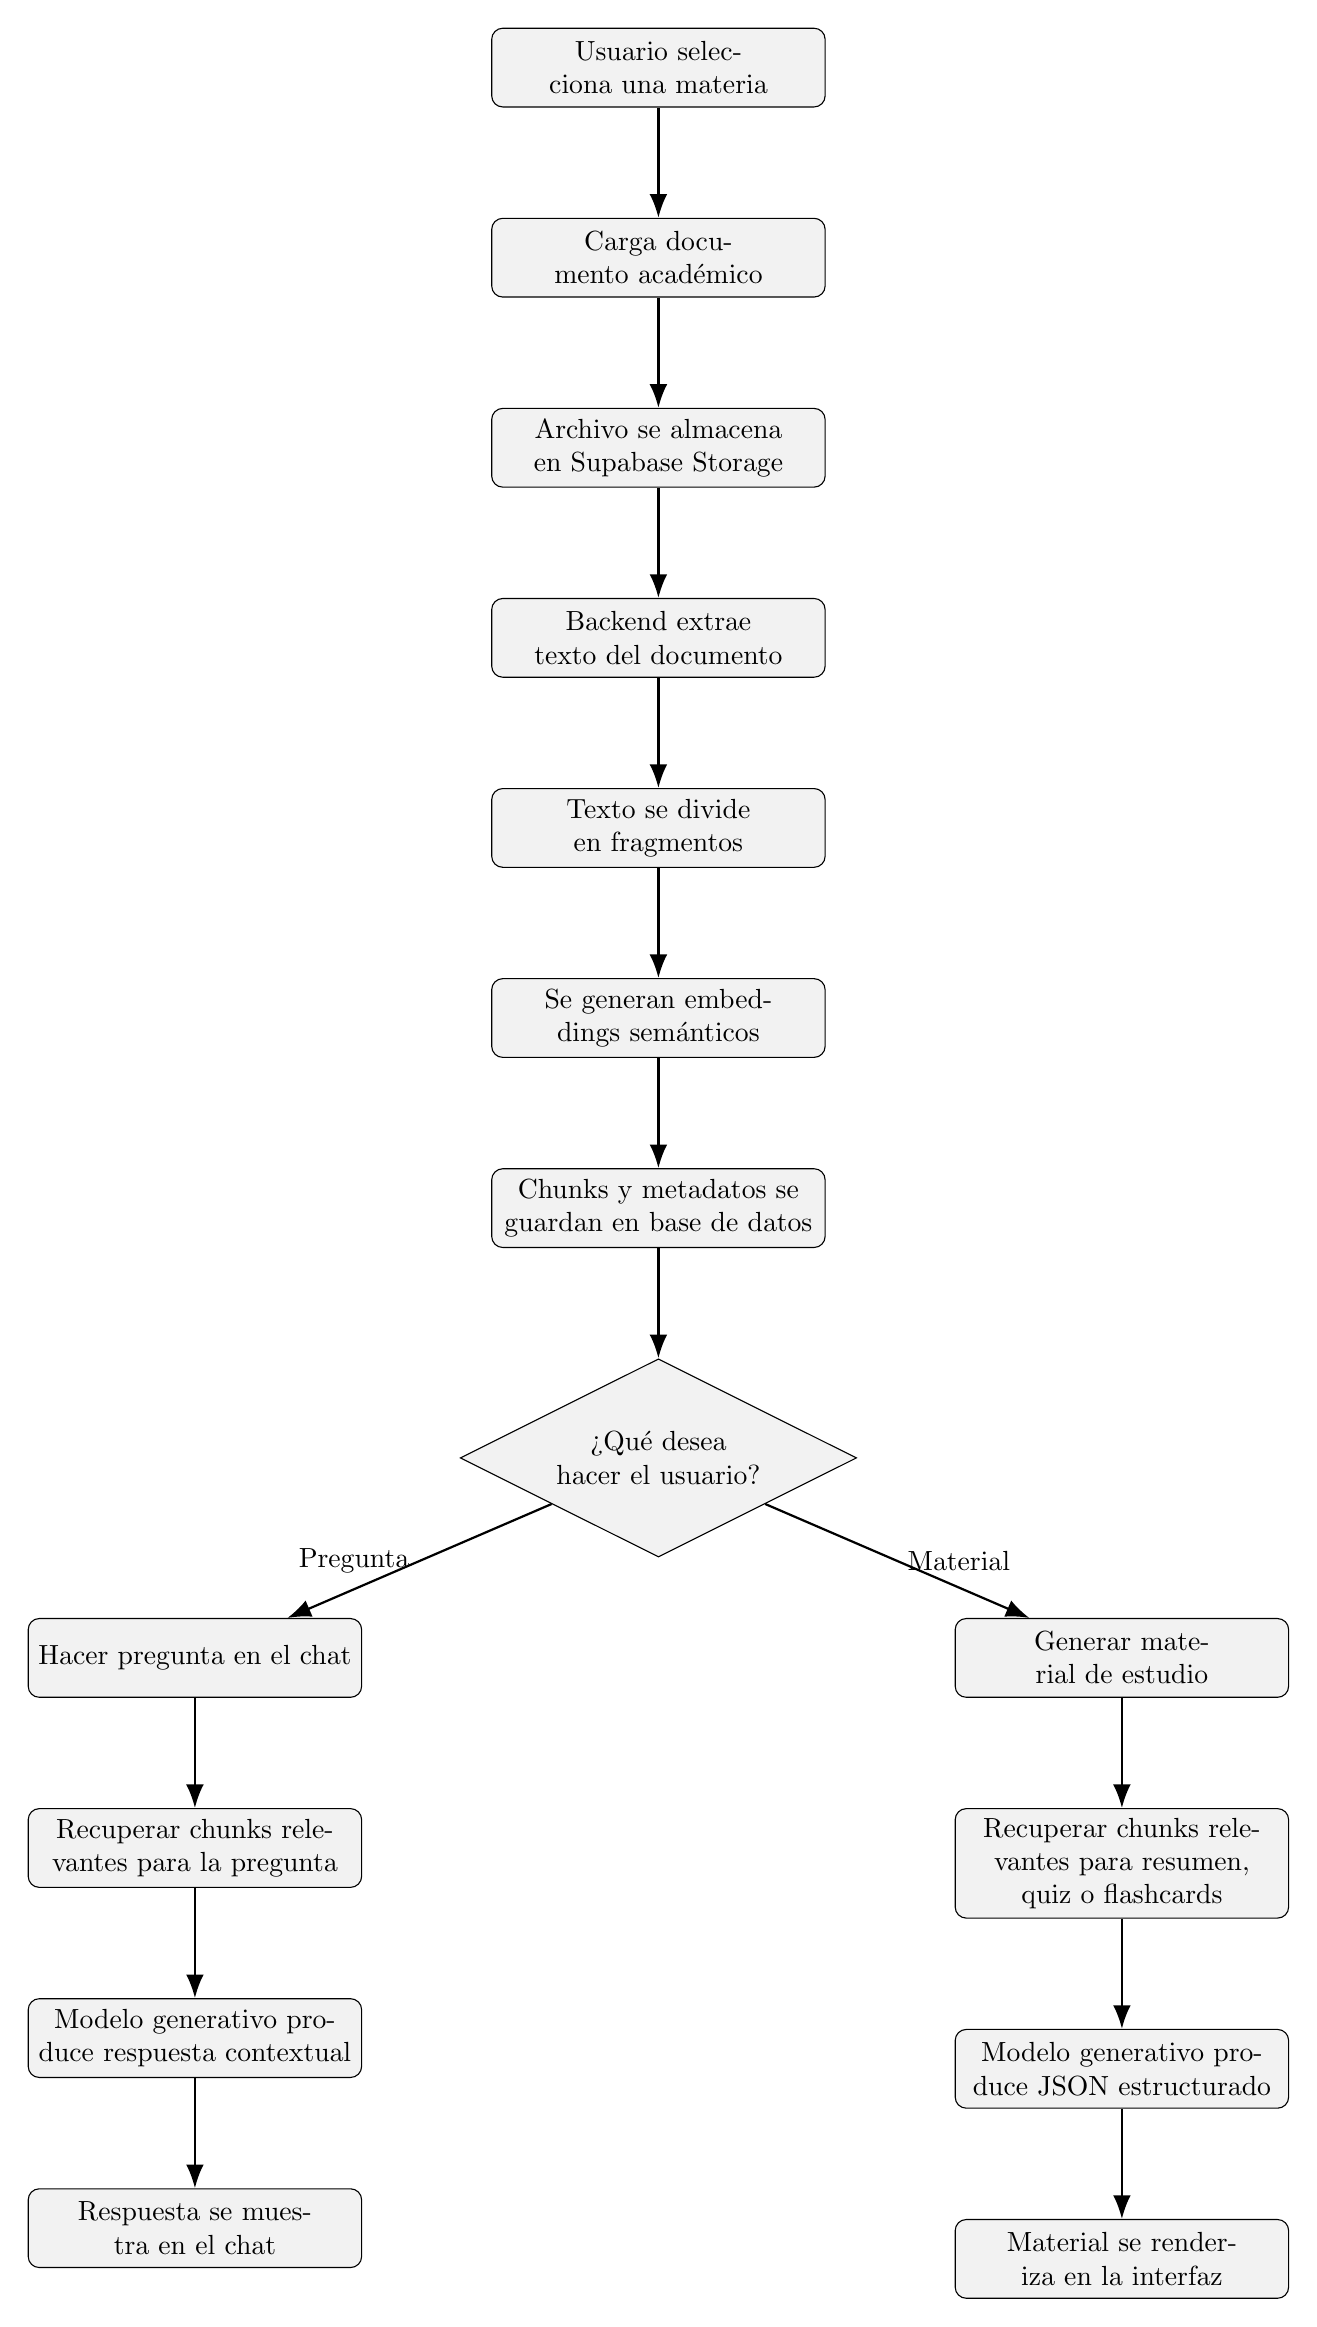
\begin{tikzpicture}[
				node distance=1.4cm,
				process/.style={rectangle, rounded corners, draw=black, fill=gray!10, text width=4cm, align=center, minimum height=1cm},
				decision/.style={diamond, draw=black, fill=gray!10, text width=3cm, align=center, aspect=2},
				arrow/.style={-{Latex[length=3mm]}, thick}
				]
				
				\node[process] (start) {Usuario selecciona una materia};
				\node[process, below=of start] (upload) {Carga documento académico};
				\node[process, below=of upload] (storage) {Archivo se almacena en Supabase Storage};
				\node[process, below=of storage] (extract) {Backend extrae texto del documento};
				\node[process, below=of extract] (chunks) {Texto se divide en fragmentos};
				\node[process, below=of chunks] (embeddings) {Se generan embeddings semánticos};
				\node[process, below=of embeddings] (db) {Chunks y metadatos se guardan en base de datos};
				\node[decision, below=of db] (action) {¿Qué desea hacer el usuario?};
				
				\node[process, below left=1.4cm and 2.5cm of action] (chat) {Hacer pregunta en el chat};
				\node[process, below right=1.4cm and 2.5cm of action] (materials) {Generar material de estudio};
				
				\node[process, below=of chat] (retrieval1) {Recuperar chunks relevantes para la pregunta};
				\node[process, below=of materials] (retrieval2) {Recuperar chunks relevantes para resumen, quiz o flashcards};
				
				\node[process, below=of retrieval1] (llm1) {Modelo generativo produce respuesta contextual};
				\node[process, below=of retrieval2] (llm2) {Modelo generativo produce JSON estructurado};
				
				\node[process, below=of llm1] (showchat) {Respuesta se muestra en el chat};
				\node[process, below=of llm2] (showmaterials) {Material se renderiza en la interfaz};
				
				\draw[arrow] (start) -- (upload);
				\draw[arrow] (upload) -- (storage);
				\draw[arrow] (storage) -- (extract);
				\draw[arrow] (extract) -- (chunks);
				\draw[arrow] (chunks) -- (embeddings);
				\draw[arrow] (embeddings) -- (db);
				\draw[arrow] (db) -- (action);
				
				\draw[arrow] (action) -- node[left]{Pregunta} (chat);
				\draw[arrow] (action) -- node[right]{Material} (materials);
				
				\draw[arrow] (chat) -- (retrieval1);
				\draw[arrow] (materials) -- (retrieval2);
				
				\draw[arrow] (retrieval1) -- (llm1);
				\draw[arrow] (retrieval2) -- (llm2);
				
				\draw[arrow] (llm1) -- (showchat);
				\draw[arrow] (llm2) -- (showmaterials);
				
			\end{tikzpicture}
		}
		\caption{Flujo general de funcionamiento de LeerIA.}
	\end{figure}
	

	\section{Desarrollo}

	
	\subsection{Descripción General de la Solución}
	
	LeerIA se desarrolló como una aplicación web compuesta por tres capas principales:
	
	\begin{itemize}
		\item \textbf{Frontend}: interfaz de usuario construida con React y Vite.
		\item \textbf{Backend}: API REST construida con FastAPI.
		\item \textbf{Persistencia}: base de datos y almacenamiento de archivos mediante Supabase.
	\end{itemize}
	
	La aplicación permite organizar el estudio por materias. Cada materia puede tener documentos, conversaciones y materiales generados. El usuario puede seleccionar una materia, subir documentos, iniciar conversaciones y generar materiales de estudio.
	
	\subsection{Conceptos de Inteligencia Artificial Utilizados}
	
	El proyecto integra varios conceptos trabajados en el curso de Introducción a la Inteligencia Artificial:
	
	\subsubsection{Procesamiento de Lenguaje Natural}
	
	LeerIA procesa documentos académicos en lenguaje natural, extrae texto y permite al usuario hacer preguntas sobre el contenido. El sistema trabaja con texto no estructurado y lo transforma en fragmentos reutilizables para recuperación y generación.
	
	\subsubsection{Recuperación de Información}
	
	El sistema usa una estrategia de recuperación de fragmentos relevantes. Cuando el usuario hace una pregunta o solicita generar material, el backend busca los chunks más relacionados con la consulta. Esto permite que el modelo no responda únicamente desde conocimiento general, sino desde el contenido documental de la materia.
	
	\subsubsection{Embeddings Semánticos}
	
	Cada fragmento del documento se representa mediante embeddings, es decir, vectores numéricos que capturan información semántica del texto. Estos vectores permiten comparar la similitud entre una pregunta y los fragmentos almacenados.
	
	\subsubsection{Modelos Generativos de Lenguaje}
	
	LeerIA utiliza un modelo de lenguaje para generar respuestas, resúmenes, preguntas de quiz, flashcards y guiones de video. El modelo recibe como entrada el contexto documental recuperado y produce una salida en lenguaje natural o en JSON estructurado.
	
	\subsubsection{RAG: Retrieval-Augmented Generation}
	
	La técnica principal utilizada es \textit{Retrieval-Augmented Generation} o RAG. Esta técnica combina recuperación de información con generación de texto. Primero se recuperan fragmentos relevantes de los documentos y luego se entregan como contexto al modelo generativo.
	
	\subsection{Arquitectura del Sistema}
	
	La arquitectura general de LeerIA se compone de los siguientes módulos:
	
	\begin{itemize}
		\item \textbf{Gestión de materias}: creación, edición y selección de materias.
		\item \textbf{Gestión de documentos}: subida, almacenamiento, procesamiento y listado de documentos.
		\item \textbf{Gestión de conversaciones}: creación de conversaciones por materia.
		\item \textbf{Chat RAG}: preguntas y respuestas basadas en documentos.
		\item \textbf{Generador de materiales}: creación de resúmenes, quizzes, flashcards y guiones de video.
		\item \textbf{Renderizado matemático}: visualización de fórmulas usando LaTeX y KaTeX.
	\end{itemize}
	
	\subsection{Tecnologías Utilizadas}
	
	\begin{table}[H]
		\centering
		\begin{tabular}{p{4cm} p{9cm}}
			\toprule
			\textbf{Tecnología} & \textbf{Uso dentro del proyecto} \\
			\midrule
			React + Vite & Construcción de la interfaz web. \\
			TypeScript & Tipado del frontend y mayor robustez en componentes. \\
			Tailwind CSS & Estilizado visual de la aplicación. \\
			FastAPI & Construcción de la API REST del backend. \\
			Supabase & Base de datos, almacenamiento de archivos y persistencia de entidades. \\
			OpenAI API / Modelo generativo & Generación de respuestas y materiales de estudio. \\
			Embeddings & Representación semántica de los fragmentos documentales. \\
			KaTeX & Renderizado de fórmulas matemáticas en la interfaz. \\
			\bottomrule
		\end{tabular}
		\caption{Tecnologías principales utilizadas en LeerIA.}
	\end{table}
	
	\subsection{Modelo de Datos}
	
	El sistema maneja varias entidades principales:
	
	\begin{itemize}
		\item \textbf{Subject}: representa una materia.
		\item \textbf{Document}: representa un archivo subido por el usuario.
		\item \textbf{DocumentChunk}: representa un fragmento procesado del documento.
		\item \textbf{Conversation}: representa una conversación asociada a una materia.
		\item \textbf{Message}: representa mensajes del usuario y del asistente.
		\item \textbf{GeneratedItem}: representa materiales generados como resumen, quiz, flashcards o guion.
	\end{itemize}
	
	Una decisión importante fue asociar los materiales generados no solo a una materia, sino también a una conversación mediante \texttt{conversation\_id}. Esto evita que diferentes conversaciones dentro de una misma materia reutilicen siempre el mismo resumen, quiz o conjunto de flashcards.
	
	\subsection{Backend}
	
	El backend está construido con FastAPI y expone endpoints REST para:
	
	\begin{itemize}
		\item crear y consultar materias;
		\item subir y procesar documentos;
		\item crear y consultar conversaciones;
		\item enviar mensajes al chat;
		\item generar materiales de estudio;
		\item recuperar artefactos generados.
	\end{itemize}
	
	El flujo de generación de material sigue esta lógica:
	
	\begin{enumerate}
		\item el usuario solicita un tipo de material;
		\item el frontend envía \texttt{subject\_id}, \texttt{conversation\_id}, tipo de material y parámetros de generación;
		\item el backend recupera fragmentos relevantes de los documentos;
		\item el modelo generativo produce una respuesta estructurada;
		\item el resultado se guarda en la tabla \texttt{generated\_items};
		\item el frontend renderiza el material en una vista especializada.
	\end{enumerate}
	
	\subsection{Frontend}
	
	El frontend incluye una interfaz dividida en tres zonas:
	
	\begin{itemize}
		\item \textbf{Sidebar izquierdo}: muestra materias y conversaciones.
		\item \textbf{Área central}: muestra chat, estado vacío, resúmenes, quizzes o flashcards.
		\item \textbf{Panel derecho}: muestra herramientas de estudio, documentos recientes y estado del sistema.
	\end{itemize}
	
	El usuario puede interactuar con LeerIA sin necesidad de usar consola ni conocer detalles técnicos del backend. Esta interfaz cumple con el requisito de interacción directa con el sistema.
	
	\subsection{Bot Conversacional de Apoyo}
	
	LeerIA incluye un bot conversacional integrado. Este bot permite hacer preguntas sobre los documentos cargados y recibir explicaciones en lenguaje natural. El bot utiliza los fragmentos recuperados como contexto para responder, lo cual reduce el riesgo de respuestas inventadas y mejora la trazabilidad hacia los documentos de la materia.
	
	\subsection{Renderizado de Matemáticas}
	
	Dado que LeerIA está orientado a documentos académicos, especialmente materias como cálculo, álgebra o estadística, se implementó soporte para expresiones matemáticas. Las fórmulas se generan en LaTeX y se renderizan en el frontend usando KaTeX.
	
	Ejemplo de una fórmula que puede ser renderizada por el sistema:
	
	\[
	\iiint_V \nabla \cdot \mathbf{F}\, dV =
	\iint_S \mathbf{F} \cdot \mathbf{n}\, dS
	\]
	
	Esto permite que el sistema sea útil no solo para textos generales, sino también para documentos técnicos y matemáticos.
	

	\section{Resultados}

	
	\subsection{Funcionalidades Implementadas}
	
	Hasta el momento, LeerIA cuenta con las siguientes funcionalidades funcionales:
	
	\begin{itemize}
		\item creación y visualización de materias;
		\item creación de conversaciones por materia;
		\item subida de documentos;
		\item procesamiento de documentos en chunks;
		\item chat con respuestas basadas en documentos;
		\item generación de resúmenes;
		\item generación de quizzes;
		\item generación de flashcards;
		\item visualización de fórmulas matemáticas en chat y materiales;
		\item separación de materiales por conversación mediante \texttt{conversation\_id};
		\item interfaz web funcional y navegable.
	\end{itemize}
	
	\subsection{Evidencia del Funcionamiento}
	
	La aplicación permite ejecutar el siguiente flujo completo:
	
	\begin{enumerate}
		\item el usuario crea o selecciona una materia;
		\item el usuario sube un documento PDF;
		\item el sistema procesa el archivo y extrae fragmentos;
		\item el usuario realiza preguntas en el chat;
		\item el sistema recupera fragmentos relevantes;
		\item el modelo genera una respuesta contextual;
		\item el usuario puede generar resumen, quiz o flashcards;
		\item los materiales generados se muestran en vistas especializadas.
	\end{enumerate}
	
	\subsection{Métricas Propuestas}
	
	Aunque el proyecto se centra principalmente en una solución funcional, se proponen las siguientes métricas para evaluar el desempeño del sistema:
	
	\begin{table}[H]
		\centering
		\begin{tabular}{p{5cm} p{7cm} p{3cm}}
			\toprule
			\textbf{Métrica} & \textbf{Descripción} & \textbf{Estado} \\
			\midrule
			Tiempo de procesamiento de documento & Tiempo desde la subida hasta la generación de chunks. & Por medir \\
			Precisión de recuperación & Proporción de chunks recuperados que realmente son relevantes. & Por medir \\
			Calidad de respuesta & Evaluación humana de claridad, fidelidad y utilidad. & Evaluación manual \\
			Consistencia del material generado & Verificación de que resúmenes, quizzes y flashcards correspondan al documento. & Evaluación manual \\
			Usabilidad de interfaz & Facilidad para completar el flujo de carga, pregunta y generación. & Validación funcional \\
			\bottomrule
		\end{tabular}
		\caption{Métricas propuestas para la evaluación de LeerIA.}
	\end{table}
	
	\subsection{Resultados Cualitativos}
	
	Durante las pruebas funcionales se observó que el sistema puede generar materiales coherentes a partir de los documentos cargados. También se identificaron y corrigieron problemas importantes, como:
	
	\begin{itemize}
		\item reutilización incorrecta de materiales generados entre conversaciones;
		\item recuperación de contexto demasiado general dentro de una materia;
		\item renderizado incorrecto de fórmulas matemáticas;
		\item necesidad de asociar materiales a conversaciones específicas;
		\item necesidad de limpiar y reforzar prompts para producir LaTeX válido.
	\end{itemize}
	
	Estas correcciones mejoraron la calidad de la experiencia de usuario y la coherencia entre conversación, documento y material generado.
	

	\section{Discusión}

	
	LeerIA se relaciona con herramientas modernas de aprendizaje asistido por inteligencia artificial, especialmente sistemas basados en RAG y asistentes conversacionales sobre documentos. A diferencia de un chatbot general, LeerIA restringe sus respuestas al contenido documental de cada materia, lo que aumenta la pertinencia para el estudio académico.
	
	El enfoque RAG ha sido ampliamente usado para complementar modelos generativos con información externa recuperada desde una base de conocimiento. En este proyecto, la base de conocimiento corresponde a los documentos cargados por el estudiante. Esta decisión permite adaptar el sistema a distintas materias sin necesidad de entrenar un modelo desde cero.
	
	Comparado con una solución de resumen tradicional, LeerIA ofrece mayor interacción porque permite preguntar, generar quizzes, crear flashcards y navegar por conversaciones. Comparado con una simple interfaz de chat, LeerIA agrega organización por materias, documentos y materiales generados.
	
	Sin embargo, el sistema también presenta limitaciones:
	
	\begin{itemize}
		\item la calidad de las respuestas depende de la calidad del texto extraído de los documentos;
		\item si los documentos tienen mala extracción OCR o símbolos matemáticos mal convertidos, el modelo puede recibir contexto imperfecto;
		\item las respuestas generadas pueden requerir validación humana;
		\item la evaluación cuantitativa del sistema aún debe fortalecerse con métricas formales;
		\item el sistema depende de servicios externos para el modelo generativo y posiblemente para embeddings.
	\end{itemize}
	
	Frente al estado del arte, LeerIA implementa una versión práctica de RAG aplicada al estudio universitario. No pretende competir con plataformas comerciales a gran escala, sino demostrar la integración funcional de conceptos de inteligencia artificial en un problema real, con una interfaz usable y un flujo completo de extremo a extremo.
	

	\section{Interfaz de Usuario}

	
	La interfaz de LeerIA fue diseñada como una aplicación web moderna e intuitiva. El usuario puede:
	
	\begin{itemize}
		\item crear materias;
		\item seleccionar conversaciones;
		\item subir documentos;
		\item escribir preguntas;
		\item recibir respuestas del asistente;
		\item generar materiales de estudio desde el panel lateral;
		\item visualizar resúmenes, quizzes y flashcards.
	\end{itemize}
	
	La interfaz cumple el requisito de interacción directa con el sistema, ya que el usuario no necesita ejecutar scripts ni manipular archivos manualmente. Todo el flujo se realiza desde la aplicación web.
	

	\section{Conclusiones}

	
	LeerIA demuestra que es posible integrar técnicas de inteligencia artificial en una herramienta educativa funcional para apoyar el estudio de documentos académicos. El sistema combina procesamiento de lenguaje natural, recuperación semántica, modelos generativos, RAG e interfaz web en una solución completa.
	
	El proyecto evidencia el uso de conceptos fundamentales del curso, especialmente procesamiento de lenguaje natural, recuperación de información y modelos generativos. Además, incluye un bot conversacional de apoyo, lo cual aporta valor adicional a la experiencia de usuario.
	
	Como trabajo futuro, se propone:
	
	\begin{itemize}
		\item implementar métricas cuantitativas de recuperación;
		\item agregar evaluación automática de respuestas;
		\item permitir selección explícita de documentos por conversación;
		\item mejorar el procesamiento de fórmulas matemáticas desde PDFs;
		\item agregar exportación de materiales generados;
		\item implementar historial de versiones de resúmenes, quizzes y flashcards.
	\end{itemize}
	

	\section{Instrucciones de Instalación y Ejecución}

	
	\subsection{Backend}
	
	\begin{lstlisting}[language=bash]
		cd Backend/LeerIA-backend
		python -m venv .venv
		source .venv/bin/activate
		pip install -r requirements.txt
		fastapi dev app/main.py
	\end{lstlisting}
	
	\subsection{Frontend}
	
	\begin{lstlisting}[language=bash]
		cd Frontend/LeerIA-frontend
		npm install
		npm run dev
	\end{lstlisting}
	
	\subsection{Variables de Entorno}
	
	El backend requiere variables de entorno para conectarse a Supabase y al proveedor del modelo generativo. Un ejemplo de archivo \texttt{.env} sería:
	
	\begin{lstlisting}
		SUPABASE_URL=...
		SUPABASE_SERVICE_ROLE_KEY=...
		OPENAI_API_KEY=...
	\end{lstlisting}
	
	El frontend requiere una URL base para la API:
	
	\begin{lstlisting}
		VITE_API_URL=http://127.0.0.1:8000/api/v1
	\end{lstlisting}
	
	
	
	
	\begin{thebibliography}{9}
		
		\bibitem{vaswani2017attention}
		Vaswani, A., Shazeer, N., Parmar, N., Uszkoreit, J., Jones, L., Gomez, A. N., Kaiser, L., \& Polosukhin, I. (2017).
		\textit{Attention Is All You Need}.
		Advances in Neural Information Processing Systems.
		
		\bibitem{lewis2020rag}
		Lewis, P., Perez, E., Piktus, A., Petroni, F., Karpukhin, V., Goyal, N., Kuttler, H., Lewis, M., Yih, W., Rocktäschel, T., Riedel, S., \& Kiela, D. (2020).
		\textit{Retrieval-Augmented Generation for Knowledge-Intensive NLP Tasks}.
		Advances in Neural Information Processing Systems.
		
		\bibitem{devlin2019bert}
		Devlin, J., Chang, M. W., Lee, K., \& Toutanova, K. (2019).
		\textit{BERT: Pre-training of Deep Bidirectional Transformers for Language Understanding}.
		Proceedings of NAACL-HLT.
		
		\bibitem{manning2008ir}
		Manning, C. D., Raghavan, P., \& Schütze, H. (2008).
		\textit{Introduction to Information Retrieval}.
		Cambridge University Press.
		
	\end{thebibliography}
	
\end{document}